\documentclass[12pt]{article}
%Gummi|065|=)
\usepackage{amsmath, amsfonts, amssymb}
\usepackage[margin=0.5in]{geometry}
\usepackage{xcolor}
\usepackage{graphicx}
%\usepackage{graphicx}
\newcommand{\off}[1]{}
\DeclareMathSizes{20}{30}{20}{18}
\newcommand{\myhrule}{}

\newcommand{\two }{\sqrt[3]{2}}
\newcommand{\four}{\sqrt[3]{4}}

\newcommand{\dash}{
\begin{tikzpicture}[scale=1]
\draw (0,0)--(19,0);
\end{tikzpicture}
}

\newcommand{\sq}[3]{
\node at (#1+0.5,#2+0.5) {#3};
\draw (#1+0,#2+0)--(#1+1,#2+0)--(#1+1,#2+1)--(#1+0,#2+1)--cycle;
}

\usepackage{tikz}

\title{\textbf{Chapter 2: Principal Component Analysis}}
\author{John D Mangual}
\date{}
\begin{document}

\fontfamily{qag}\selectfont \fontsize{15}{20}\selectfont

\maketitle

\noindent Machine learning is just linear regression and best fit lines.  And that is just the Pythagorean theorem.  Today let's discuss \textbf{Principal Component Analysis}. \\ \\
Our data points are $x^{(1)}, \dots, x^{(m)} \in \mathbb{R}^n $ so we can merge them into a single matrix $X \in \mathbb{R}^{m \times n}$.
$$ \begin{tikzpicture}  
\draw (0,0)--(1,0)--(1,5)--(0,5)--cycle; 
\node at (0.5,2.5) {$x^{(1)}$};

\node at (1.5,2.5) {$\oplus$};

\draw (2,0)--(3,0)--(3,5)--(2,5)--cycle; 
\node at (2.5,2.5) {$x^{(2)}$};

\node at (4,2.5) {$\oplus \dots \oplus $};

\draw (5,0)--(6,0)--(6,5)--(5,5)--cycle; 
\node at (5.5,2.5) {$x^{(n)}$};

\node at (6.5,2.5) {$=$};

\draw (7,0)--(10,0)--(10,5)--(7,5)--cycle;
\node at (8.5,2.5) {$X$};

\end{tikzpicture} $$
In Python is this done with the \texttt{np.hstack} or \texttt{np.vstack} commands (where \texttt{numpy} is shortened to \texttt{np}). \\ \\
In beginning statistics we search for the best fit line.  That means all our data points $x$  approximately solve the same equation:
$$ A x + B \approx 0 $$ 
What are the dimensions of $A$ and $B$?  Our vectors $x$ have shape $1 \times n$ and the zero has shape $1 \times 1$, so that $A$ has shape $n \times 1$ and $B$ has shape $1 \times 1$.  However, reduction to a line may lose much information.  \\ \\
What if we need more features?  Let's take $n_0 < n$ feature. \\ \\
What are the dimensions of $A$ and $B$?  Our vectors $x$ have shape $1 \times n$ and the zero has shape $1 \times n_0$, so that $A$ has shape $n \times n_0$ and $B$ has shape $1 \times n_0$.  

\newpage

\noindent What is a reasonable numbe of data points?  Some data sets brag as much as a billion, $m = 10^9$ data points.  Each row of data could have as much as $n = 100$ features (or more) and we could like to reduce that to $n_0 = 10$. \\ \\
If our data set included a few bit of inforation about each person:
\begin{itemize}
\item Height
\item Favorite Ice Cream
\item {\color{black!20!white} Birthday}
\item {\color{black!20!white} Occupation}
\end{itemize}
Can we infer the \textbf{Birthday}  and \textbf{Occupation} from the height and favorite ice cream flavor?  Hopefully there is some type of {\color{green!20!blue}correlation}! \\ \\
So we will take our data points $X$ and find the covariance matrix.  Hopefully our numbers do not have too much mistakes because they may propagage throughout our computation!
$$ \text{Covariance} = X^T X  \in \mathbb{R}^{m \times m}$$
What is the shape of our matrix?  It is always okay to multiply a matrix with its own transpose:
$$ (m \times n ) \cdot (n \times m) = m \times m \quad\text{ or }\quad(n \times m) \cdot (m \times n) = n \times n$$
$n$ is the \textbf{number of features}  and $m$ is the \textbf{number of data points}, so we are doing the one on the right.  \\ \\
 Next we decide which features are the most important.  Using the eigenvalue decomposition:
$$ X^T X \sim \left[ \begin{array}{cccc} \lambda_1 & & & \\ & \lambda_2 & & \\ &  &  \ddots  \\ 
& & & \lambda_n \end{array} \right] $$
Our matrix is not only square, but they are symmetric!  So the eigenvalues $\lambda \in \mathbb{R}$ can be compared.
$$ \lambda_1 > \lambda_2 > \dots > \lambda_n $$

\newpage

\noindent An example of a matrix whose eigenvalues cannot be a real number is a \textbf{rotation} by $90^\circ$: 
$$ \left[ \begin{array}{cr} 0 & -1 \\ 1 & 0 \end{array}\right] 
\sim \left[ \begin{array}{cr} \sqrt{-1} & 0 \\ 0 & \sqrt{-1} \end{array}\right] $$
Here is a $2 \times 2$ matrix which is not diagonal.  There is only one eigenvector:
$$ \left[ \begin{array}{cr} 1 & 1 \\ 1 & 0 \end{array}\right] $$
This is called a \textbf{shear}.  \\ \\
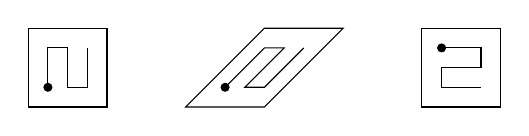
\begin{tikzpicture}

\draw (0,0)--(1,0)--(1,1)--(0,1)--cycle;
\draw (0.25,0.25)--(0.25,0.75)--(0.5,0.75)--(0.5,0.25)--(0.75,0.25)--(0.75,0.75);
\draw[fill=black] (0.25,0.25) circle (0.05);

\begin{scope}[cm={1,0,1,1,(2,0)}]
\draw (0,0)--(1,0)--(1,1)--(0,1)--cycle;
\draw (0.25,0.25)--(0.25,0.75)--(0.5,0.75)--(0.5,0.25)--(0.75,0.25)--(0.75,0.75);
\end{scope}
\draw[fill=black] (2.5,0.25) circle (0.05);

\begin{scope}[cm={0,-1,1,0,(5,1)}]
\draw (0,0)--(1,0)--(1,1)--(0,1)--cycle;
\draw (0.25,0.25)--(0.25,0.75)--(0.5,0.75)--(0.5,0.25)--(0.75,0.25)--(0.75,0.75);
\draw[fill=black] (0.25,0.25) circle (0.05);
\end{scope}

\end{tikzpicture}\\ \\
Our covariance matrix is symmetric: $(X X^T)^T = X^T (X^T)^T = X X^T$, so out our eigenvalues, our {\color{green!20!blue} \textbf{features}} are real numbers.  In practice these features will be linear combinations and therefore totally ridiculous:
$$ \frac{1}{2} \times \text{Height} + 2 \times \text{Birthday} $$
Let us proceed with our analysis of Principal Component Analysis.\\ \\
The goal of PCA is to somehow ``shrink" the data in to more mangeable form.  This could be:
\begin{itemize}
\item shrinking an image file using JPEG, PNG, GIF or some other file format
\item shrinking a WAV file to MP3
\item shrinking a video to fit on your mobile phone
\end{itemize}
All of these compressions can be modeled as linear transforms from a space of $n \times 1 $ vectors to smaller $n_0 \times 1$ vectors:
$$ f: x \in \mathbb{R}^n \mapsto c \in \mathbb{R}^{n_0} $$
and this is what we call a \textbf{lossy} compression (or a ``matrix").  How could it be possible to keep all this information?  We simply cannot. \\ \\
If we are lucky there will be some correlation and we can recover some of the information we have lost. $x = g(c) $ and $c = f(x)$ with $x \approx (g \circ f)(x)$ 

\newpage

\noindent Our deep learning textbook has two simplifications that $f$ and it's ``pseudoinverse" $g$ are both linear transformations:
\begin{itemize}
\item $c = f(x) = D\;\,x$
\item $x = g(c) = D^T x$
\item $x = (g \circ f)(x) $
\end{itemize}
It will be impossible to have all these true for all our data points, so what is the best we can do? \\ \\
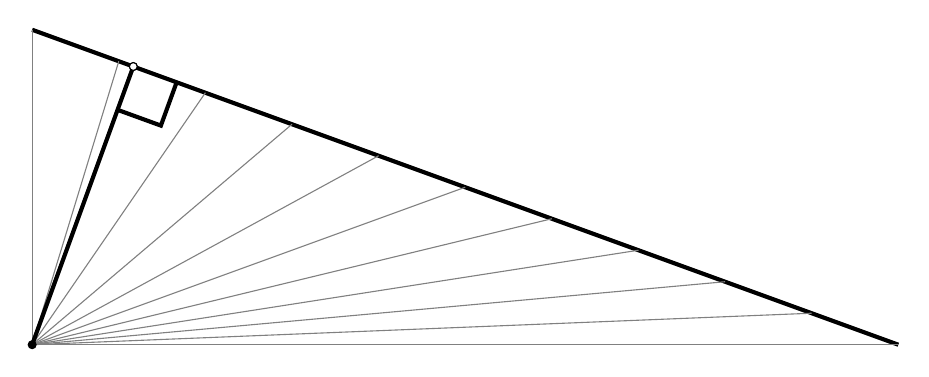
\begin{tikzpicture}



\draw[line width=1.5] (11,0)--(0,4);

\foreach \a in {0,...,10}{
	\draw[color=black!50!white] (0,0)--( 11- 11*\a/10 , 0 + 4*\a/10 );
}

\draw[line width=1.5] (0,0)--(4*4*11/137, 4*11*11/137);
\draw[fill=black] (0,0) circle (0.05);
\draw[fill=black] (4*4*11/137, 4*11*11/137) circle (0.05);
\draw[fill=white] (4*4*11/137, 4*11*11/137) circle (0.05);

\draw[line width=1.5] (4*4*11/137 + 11*0.05 , 4*11*11/137 - 4*0.05)--(4*4*11/137 + 11*0.05 - 4*0.05 , 4*11*11/137 - 4*0.05 - 11*0.05)--(4*4*11/137 - 4*0.05 , 4*11*11/137 - 11*0.05);

\end{tikzpicture} \\ \\
The closest point from one point to the line can be found by dropping a perpendicular.  Even if a curve, the tangent line will be perpendicular. \\ \\
If there are many points, then we have many points we can drop to a particular line.  And we want the sum of the squares of all these distances.

\includegraphics[width=7in]{linear-algebra-01.png}

\noindent We include some random points and a candidate best fit line.

\newpage

\noindent Ng's Coursera course \textit{agonizes} over best fit line, since he knows I am right.

\includegraphics[width=7in]{linear-algebra-02.png}

\noindent This example is not the most aesthetic, just like real data is not. \\ \\
Which one is a better fit? 

\newpage

\noindent Let's do some basic linear algebra (despite its simplicity it took a long time):

$$ x \in \mathbb{R}^N \stackrel{f}{\mapsto} c = f(x) \in \mathbb{R}^M \stackrel{g}{\mapsto} x \approx (g \circ f)(x) \in \mathbb{R}^N $$
This looks just like inverse functions, but if $M \gg N$ there can be no inverse that works everywhere.  This is why we need a \textbf{pseudoinverse}.  I don't even know the definition. \\ \\
Let's construct one a pseudoinverse by finding the constraints.
$$ x \in \mathbb{R}^N \stackrel{f}{\mapsto} D \, x \in \mathbb{R}^M \stackrel{g}{\mapsto} x \approx D^T D \, x \in \mathbb{R}^N $$
and if $x$ lies perfectly on the best-fit line (or best fit linear subspace)
$$ D^T D = I_{M \times M} $$
This is a \textbf{rotation} (or ``orthogonal matrix").  Except this $D$ is an $N \times M$ matrix up to rotations, so this is an element of the Grassmanian.\footnote{https://en.wikipedia.org/wiki/Grassmannian} \\ \\
Why did we pick the transpose?  We are trying to solve a minimization problem:
$$  \min \big|\big| x - (g \circ f)(x) \big|\big|^2 $$
If we decide the decoder function is $g(c)= D \, c$, we can try to solve this simplified problem. 
$$ \min_c \big|\big| x - D \, c \big|\big|^2 $$
The closest we can get to an inverse is by the transpose, $c = f(x) = D^T x$. \\ \\
{\color{blue!20!green!70!white}\textbf{Best Fit Hyperplane}} I am trying to find a way of encoding my length $N$ with less information, just $N$ bits and it should work reliably on all my existing data points.  So I am going to guess that all my points live on an $M$ dimensional subspace.
$$ \mathrm{Gr}(N,M) = O(N)/\big( O(M) \times O(N-M) \big) $$
and $D$ is an element of this Grassman space.  And we would like to minimize the error obtained over all possible choices of $D$:
$$ \min_D \big|\big| x - (D^T D ) x \big|\big|^2 = 
\min_D \bigg|\bigg| x \, \big(I - (D^T D )\big)  \bigg|\bigg|^2 
$$
To me this is just another $L^2$ norm. The Grassmanian is compact and there must be a minimum, found by a method of your choice.
 
\newpage

\noindent Then we can prove the minimizing $D$ is found by in fact the covariance of our data points $X^T X$.  And we can prove that any flow on the Grassmanian (such as \textbf{stochastic gradient descent}) \\

\fontfamily{qag}\selectfont \fontsize{10}{15}\selectfont

\noindent If I google the phrase ``{\color{blue!50!green}principal component analysis grassmanian}" more than zero things arise. Including this one:
\begin{itemize}
\item Matthew Nokleby, Miguel Rodrigues, Robert Calderbank \textbf{Discrimination on the Grassmann Manifold: Fundamental Limits of Subspace Classifiers} \texttt{ arXiv:1404.5187}
\end{itemize}
I don't want to be stuck analyzing giant spreadsheets all day, when we all have things we want to do.  At least someone has observed the geometric approach to PCA, that I am advocating. 
\end{document}
